% !TEX root = ./paper.tex
% Design note to remember to explain: multi-stream \tcpls must increase the lower
% 64 bits of the IV to keep using a counter starting a 0. (though, we need a
% limit on the number of paralel stream creation)

\subsection{The Secure Control Channel}\label{sec:extending}

\tls 1.3~\cite{rfc8446} has been designed with careful consideration for
potential extensions and to prevent middlebox interference.  A \tcpls client
indicates its willingness to use \tcpls with a transport parameter in the
\textsc{ClientHello} message. Upon reception of this parameter, the server
replies with a \textsc{ServerHello} messages. It can opportunistically as
lightweight \tcpls data and \tcp options as \textsc{EncryptedExtensions}. Any
extension sent with the \textsc{ServerHello} message is encrypted with the
handshake key, and is not part of the context used to derive the eventual
application key. If the client does not support some extension, it echoes back
an alert with the value of the option it does not recognize, but the connection
continues.

A reasonable approach to designing extensibility mechanisms in today's Internet
is to avoid leaking any information that could help an on-path attacker
recognize specific users or applications. Indeed, censorship~\cite{Morshed2017a,
Gosain2017a,Chai2019a} can be easily implemented when protocol messages can be
distinguished, and avoiding trivial opportunities to implement censorship should
become the bare minimum in designing a new protocol. \tcpls's control protocol
considers those problems by avoiding unencrypted data within the
\textsc{ClientHello}.

Once the secure handshake has succeeded, the hosts can exchange \tls records.
To prevent middlebox interference, the \tls 1.3 Record Protocol ensures that any
new message appears as an \textsc{AppData} message type while the true content
type (TType) is stored at the end of the encrypted payload. \tcpls uses this
feature of \tls 1.3 to encode the control messages that are sent over the secure
channel as new \tls record types.

%It supports the \textsc{EncryptedExtensions} message sent
%by the server alongside the \textsc{ServerHello}.
%Such a design choice eases dealing with implementations
%not supporting a particular option since an opportunistic transmission
%of an option will not affect the handshake outcome.


%\tls 1.3~\cite{rfc8446} defines several types of \tls messages.
%\tcpls relies on several of them.
%A \tcpls client indicates its willingness to use \tcpls with a
%transport parameter in the \textsc{ClientHello} message.

\subsection{The \tcpls Streams}\label{sec:datastreams}
%%%%%%%%%%%%%%%%%%%%%%%%%%%%%%%%%
The classical solution to support streams in a transport protocol is to assign
an identifier to each stream and send the data from stream $x$ as a tuple
$x,seq,data$ where $seq$ is a sequence number. This is the solution chosen by
\sctp~\cite{rfc4960} and \quic~\cite{draft-ietf-quic-transport}. \tcpls relies
on cryptographic properties to support several streams.

\paragraph*{Cryptographic Details and Tricks} In \tcpls, each stream has its own
cryptographic context. All streams use the same key but derive a specific
Initial Vector (IV - also called cryptographic nonce) such that nonce-misuse
cannot happen. Furthermore, we derive the IV such that \tcpls record sequence
number can securly start at $0$ within each stream.

\tcpls uses only one application-level key for $N$ streams, for each direction.
We selected this approach is to avoid security degradation with the usage of
multiple keys (by a factor $k$ with $k$ keys)~\cite{chatterjee2011another}.

To enable all stream sequence numbers to start at 0, we rely on some properties
of the Authenticated Encryption with Associated Data (AEAD) schemes used by \tls
1.3. To preserve AEAD security, the AEAD nonce used by \tcpls must be of unique
use when encrypting and decrypting a record. The initial nonce must also be
unpredictable for an adversary observing the handshake. \tcpls derives it from
the \tls handshake session secret in a similar fashion as the \tls
keys~\cite{rfc8446}. The nonce size must range from $96$ bits to $128$ bits
depending on the underlying cipher used. In all cases, for a nonce of size $N$
bits, \tls computes the cryptographic nonce given to the underlying by
concatenating the $N-64$ leftmost bits with the 64 lower bits xored with the
record's implicit sequence number encoded in 64 bits.  The lower 64 bits xoring
provides more unpredictability to the nonce when the same plaintext is encrypted
multiple times with the same key~\cite{bellare2016multi,hoang2018multi}. This
design implies that we give to the underlying cipher the 32 upper bits
untouched. The resulting value is then incremented at most 1024 times starting
from the leftmost bits to encrypt a \tls record of maximum size (16384 bytes,
i.e, 1024 times 128 bits for the the
minimum block size). We thus observe that 7 bits among those 32 bits are
untouchable, leading to at least 25 bits that are available to encode a unique
stream number. By encoding such a unique number in this part of the
cryptographic nonce, we enable each stream to start its sequence number at 0
while encrypting its records with the same key. This observation means that we
can create independant cryptographic contexts based on a tweak of the
cryptographic nonce. This implies that stream records can be encrypted and
decrypted independently of each other, with the same key value. This technique
maintains AEAD's core assumption (uniqueness of nonce), which means that the
state of art AEAD's security proof starting from that assumption applies to our
design~\cite{chatterjee2011another} and guarantees the security of our scheme.

\paragraph*{Carrying Multiple Streams over the Same Transport}
Thanks to those separate cryptographic contexts, \tcpls can perform concurrent
encryption and decryption between streams while maintaining decryption
correctness and security, and potentially also use this capability to process
streams over multiple cores. Finally, if different streams are carried
over the same \tcp connection, \tcpls does not explicitely know which
received record belongs to which stream. To retrieve this information,
we also
%either require to modify the
%associated information within \tls records to add a stream id (this associated
%data is not encrypted but the AEAD cipher authenticates them). This choice
%means potential middlebox interference, which we chose to avoid. The other
%option is to
leverage the AEAD cipher and check the authentication tag of the incoming record
until we find the stream that properly verifies this tag. This operation is
lightweight: it does not require full decryption of the record because the AEAD
ciphers used by \tls 1.3 do Encrypt then MAC (and MAC then Decrypt). This
implies that they first check the tag and only decrypt if the tag is correct.
Looking for the right stream that succeeds the tag verification needs to be
performed once each time the application writes to another stream over the same
\tcp connection.

Note that, security-wise, each failed decryption is considered as a
forgery attempt. However, we have large limits on the confidentiality and
integrity with all AEAD ciphers~\cite{luykx2015limits, aeadlimits} before a
successful forgery may be considered as a non-negligeable probability. For
example, in the case of ChaCha20+Poly1305, an adversary making $2^{60}$ forgery
attempts succeeds with probability $2^{-33}$.

%Streams are an interesting abstraction for applications. Experience with HTTP/2
%has shown that head-of-line blocking was an important factor in web performance.
%This motivated the first QUIC design \cite{langley2017quic}. If all data streams
%are mapped on the same underlying \tcp connection, head-of-line blocking remains
%possible. However, this blocking can be prevented by using different \tcp
%connections to transport the different data streams.


\subsection{Connection Management}
\label{sec:multipath}

\tcpls includes a Connection Manager (CM) that controls the underlying \tcp
connections.
%In our design mindset, Multipath in a modern transport protocol is about
%offering all the performance and usability opportunities we can imagine from
%multiple interfaces and network paths, in a fully flexible manner with a clear
%justification for what is internal to the stack, and
The CM is fully configurable and exposed to application developers.
\tcpls enables the client or the server to associate new \tcp connections to an
existing \tcpls connection. This is similar to \mptcp's path managers
does~\cite{raiciu2012hard,rfc6824,hesmans2015smapp,hesmans2016enhanced},
but with some differences. First, \tcpls does not suffer from the same
security limitations as \mptcp. Second, \tcpls supports several modes
of multipathing including connection failover and bandwidth aggregation.



\begin{figure}[!t]
  \centering
  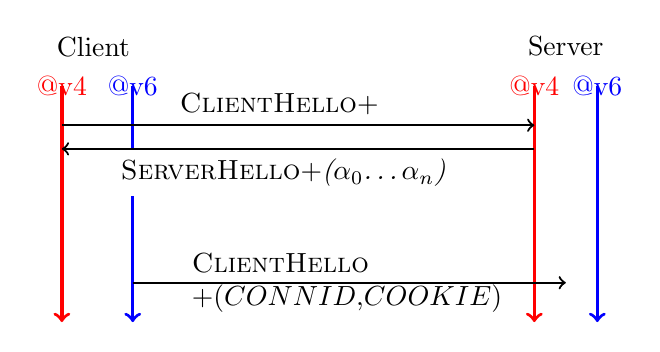
\begin{tikzpicture}
    \colorlet{lightgray}{black!20}
    \tikzstyle{arrow} = [thick,->,>=stealth]
    \tikzset{state/.style={rectangle, dashed, draw, fill=white} }
    \node[black, fill=white] at (0,10) {Client};
    \node[black, fill=white] at (6,10) {Server};
    \node[red, fill=white] at (5.6,9.5) {@v4};
    \node[blue, fill=white] at (6.4,9.5) {@v6};
    \node[red, fill=white] at (-0.4,9.5) {@v4};
    \node[blue, fill=white] at (0.5,9.5) {@v6};
    \draw[red, very thick,->] (-0.4,9.5) -- (-0.4,6.5);
    \draw[blue, very thick,->] (0.5,9.5) -- (0.5,6.5);
    \draw[red, very thick,->] (5.6,9.5) -- (5.6,6.5);
    \draw[blue, very thick,->] (6.4,9.5) -- (6.4,6.5);
   \draw[black, thick, ->] (-0.4,9) -- (5.6,9) node [midway, fill=white, above,
   text width=3cm] {\textsc{ClientHello}+\emph{\tcpls}};
   \draw[black, thick, <-] (-0.4,8.7) -- (5.6,8.7) node [midway, fill=white, below, text width=4.5cm] {\textsc{ServerHello}+\emph{\tcpls($\alpha_0$\ldots$\alpha_n$)} };
   \draw[black, thick, ->] (0.5,7) -- (6.0,7) node [midway, %fill=white, above,
   text width=4cm] {\textsc{ClientHello}\\+\join($CONNID$,$COOKIE$)};
  \end{tikzpicture}
  \caption{\tcpls supports the attachment of additional \tcp
    connections to a \tcpls connection. Each $\alpha_i$ is encrypted with the
    handshake key.}
  \label{fig:join-example}
\end{figure}

\paragraph*{1) Better Security Than \mptcp} A \mptcp connection gathers several
underlying connections that are called subflows. To ``secure'' the attachment of
additional subflows, \mptcp hosts exchange short keys in plaintext inside \tcp
options during the \tcp handshake~\cite{rfc6824, rfc8684}. These keys are then
used later to authenticate the attachment of subflows to a connection. An
attacker that has observed the initial handshake can attach any subflow to an
existing \mptcp connection~\cite{rfc6181}.  \tcpls solves this
\texttt{``connection join''} problem in a much more secure mmanner. Consider a
client connecting to a dual-stack server. Fig.~\ref{fig:join-example} depicts
the \tls messages exchanged. The client sends a \textsc{ClientHello} containing
the \tcpls extension to negotiate \tcpls.  The server replies with a
\textsc{ServerHello} with three types en encrypted extensions. \todo{$alpha$
  adapter}. First, the server announces its IPv4 and IPv6 addresses. Second, it
associates one identifier to the \tcpls session.  This identifier uniquely
identifies the \tcpls session on the server.  Third, the server provides a list
of \tcpls session cookies. Each of these session cookies enables the client to
attach one additional \tcp connection to the \tcpls session. By sending $n$
cookies, the server indicates that it currently accepts the attachment of only
$n$ \tcp connections to this session. This prevents resources exhaustion attacks
that are difficult to counter with \mptcp. \todo{OB:voir mpquic} The server can
send additional cookies later and update its list of addresses. \tcpls is
symmetrical and the client can also announce its addresses and send cookies.

To attach a new connection, e.g., using the server's IPv6 address, the client
sends a \textsc{ClientHello} message containing the session identifier
($SESSID$) and one of the server's cookies ($COOKIE$). The server checks the
validity of the cookie and then uses the session identifier to attach the new
\tcp connection to the right \tcpls session. The session identifier and cookie
play that same role as \mptcp's token. From a security viewpoint, the session
cookie is longer than \mptcp's token. Furthermore it is sent encrypted in the
initial \textsc{ServerHello} message, and can only be used once (i.e., when the
server receives a valid cookie, it accepts the connection, attaches it to the
right \tcpls session, and discard the cookie).

%Thanks to the cookies, the server can limit the number of \tcp connections that
%a client can attach to a \tcpls connection. Apart from preventing on-path
%attackers to join the connection like in \mptcp, this also prevents some
%denial-of-service attacks. \fr{Which ones?}

\paragraph*{2) Flexible Connection Migration} \tcpls supports two mode of
connection migration. First, the Failover mode.  This Failover is fully internal
to \tcpls and similar to \quic's connection migration and \mptcp's failover:
upon network outage, \tcpls can recover the session over another \tcp
connection. When the failover mode is enabled, \tcpls sends stream-level record
acknowledgments that announce to the peer the records that have been received
over each stream.  Upon network outage, \tcpls \textbf{\textit{moves}} the
active streams out of the broken \tcp connection to an active one. Furthermore,
the unacknowledged data records that were sent over a failed \tcp connection are
\textbf{\textit{sent again}} on a functional \tcp connection.
%\todo{FR OB ne comprend pas la phrase qui suit} Moving the streams involves
%playing a protocol that we designed to re-synchronize the implicit stream-level
%sequence number that is used to encrypt and decrypt records.
\tcpls' Failover mode is optionnal. It needs to be activated by both peers.  We
discuss in Sec.~\ref{sec:perf} measurements that quantify the performance impact
of this mode.

Second, \tcpls also supports \textit{Application-level Connection Migration}.
Essentialy, it means that \tcpls provides a simple API that enables an
application to migrate when it wishes to do so (e.g., a smartphone could migrate
from LTE to Wi-Fi when the Wi-Fi appears healthy, a client using privacy
compliant IPv6 addresses \cite{rfc4941} could restart the underlying \tcp
connection after the expiration of a temporary address, \ldots). The semantic of
the application-level connection migration is built from attaching and
closing streams in the multipath bandwidth aggregation mode.
The host that wishes to carry such a migration first creates a new \tcp
connection and join the \tcpls session over this connection. Then, it
attaches new streams to the new connection by sending one
\texttt{STREAM\_ATTACH} message per stream that needs to be migrated. At that
moment, the client and the server have potentially multiple streams opened over
the two network paths. Then, after attaching its streams to the new path, the
migrating host sends a \texttt{STREAM\_CLOSE} message over the old \tcp
connection for all old streams. At this point, the migrating host cannot send new data anymore for
the streams over the old connection. Once the remote host has received a
\texttt{STREAM\_CLOSE} message over the old \tcp connection, it knows that the
stream is not available anymore, and needs to find a (potentially fresh) stream to send its
data (i.e., the ones that just opened over the new path). It first sends a
\texttt{STREAM\_CLOSE\_ACK} message for each received \texttt{STREAM\_CLOSE}.
The migrating host can close the old connection upon reception of the last
\texttt{STREAM\_CLOSE\_ACK}, indicating that no more data would be received over
this connection. Note that since these messages are TLS records, they are sent
reliably by the underlying \tcp connection.

This second type of migration does not require application-level
acknowledgements, but it cannot survive from the failure of one of the
underlying connections. During such a migration, some data is sent over two
connections, which brings us to explain how multipath is designed

%Compared to \quic's connection migration and \tcpls's failover,
%this migration does not has no goodput loss. It even temporaly increases the goodput by aggregating the
%bandwidth of both interfaces until the first stream has flushed all its data
%(depending on the data left in \tcp's sending buffer and the path bandwidth and
%latency when the migration starts).  That is, in this specific use case,
%bandwidth aggregation is only used during the migration to ensure a smooth
%transition, and once \tcpls has migrated, we are back to one path. In comparison
%to the Failover mode, this mode does not require acks to be exchanged, neither
%both peers must agree on the functionality. However, it cannot survive a network
%outage.


\paragraph*{3) Different Multipath Modes}
Like \mptcp \cite{raiciu2012hard,rfc6824} or Multipath QUIC \cite{viernickel2018multipath,de2017multipath,draft-deconinck-quic-multipath-06,draft-liu-multipath-quic-02}, \tcpls supports an aggregation mode that maps data over two or more \tcp connections. On multihomed hosts, this can increase the total throughput of a \tcpls session by spreading the data over different network interfaces. In this case, one or more data streams are mapped to two or more underlying \tcp
connections and \tcpls schedules different records over different connections.

In addition, \tcpls allows the application to attach its streams to the
underlying \tcp connections in a non-aggegated bandwidth mode.
This is a choice left to the application using the API. It has several
advantages and inconvenients compared to the aggregation mode. For example, the
aggregation mode is simple to use and can potentially saturate the available
network paths but can lead to Head-Of-Line (HOL) blocking,
since packets sent over different \tcp connections need to be eventually
re-ordered. The aggregation mode is also more CPU
costly, since a zero-copy codepath is technically possible only when the packets
arrive in order. In the non-aggregated multipath mode, the application needs to
take care to fully send an application-level object over the same stream, since
the ordering is only guaranteed per-stream in this mode. However, our \tcpls
implementation guarantees that this mode will benefit from zero-copy of the decrypted application data, which
makes this mode potentially quite interesting for application protocol such as
HTTP that needs to fetch multiple application objects at the same time.

\subsection{Improving \tcp's Extensibility}
\todo{move to appendix ?}
\label{sec:tcpoptions}
% Discussing the lack of extensibility of TLS 1.3;
\begin{figure}[!t]
  \begin{bytefield}[bitwidth=0.47em]{40}
    %\bitheader[lsb=0,bitformatting={\tiny\rotatebox[origin=B]{90}}]{0,7,8,15,16,23,24,31,32,39} \\
    \bitheader[lsb=0,bitformatting={\tiny}]{0,7,15,23,31,39} \\
    \begin{rightwordgroup}{Header}
      \bitbox{8}{Type} & \bitbox{16}{Version} & \bitbox{16}{Length}
    \end{rightwordgroup}\\
    \begin{rightwordgroup}{Payload}
      \bitbox{16}{Option Type} & \bitbox{16}{User Timeout} & \bitbox{8}{TType}
     %&\wordbox[lrb]{1}{Padding... (to match the AEAD block size)}
    \end{rightwordgroup}\\
  \end{bytefield}
  \caption{A new type of \tls Record containing a \tcp option.}
  \label{fig:ex_record}
\end{figure}

\tcp \cite{rfc793} limits the size of the entire \tcp header (including options) to 64 bytes. Unfortunately, the \tcp designers did not foresee that so many \tcp extensions would be standardized. Today, the size of the \tcp header
becomes a constraint.
%For example, it severely limits the number of gaps that
%can be covered by selective acknowledgments.
This gets worse with extensions
such as \mptcp~\cite{rfc6824} that consume more space in the \tcp header.
The IETF has discussed this problem for several years, but the latest attempt
to solve it~\cite{draft-ietf-tcpm-tcp-edo-10} has not yet been implemented by
major \tcp stacks.

\tcpls provides more space for some \tcp options. First, with \tcpls, \tcp
options can be negotiated during the \tls handshake. Since the \tls messages are
included in the \tcp payload, there is more space to carry them. Another
advantage of this approach is that the \tcp options are secured by \tls. This
implies that they cannot be modified by middleboxes. This could be an advantage,
but could also prevent \tcpls from correctly working through some types of
transparent \tcp proxies.

Second, \tcpls can also carry \tcp options inside \tls records. \tcpls includes
one record type to carry TCP options. This new type of records can be used to carry TCP options that need to be exchanged reliably such as the \tcp User Timeout option \cite{rfc5482} or \mptcp's \texttt{ADD\_ADDR} and \texttt{REMOVE\_ADDR} option or experimental TCP options \cite{rfc6994}.

%For example, we used
%this feature to implement the Linux \tcp User Time Out option
%(Figure~\ref{fig:ex_record}). A client
%can use this option to set the maximum value of the retransmission
%timer on a server. Linux \tcp has a socket option that allows setting
%this timer locally, but it does not implement let the stack carry this \tcp
%option to the other peer. With \tcpls, the client sends the option inside a \tls
%record, the server extracts it and performs the required \texttt{setsockopt}.


\subsection{Secure Connection Closing}

\tcpls's semantic offers a secure stream abstraction to the application.
Streams can be attached to and closed from what we call a \texttt{transportid}
(the application does not have knowledge of the \tcp interface). When a stream
gets attached for the first time to a \tcp connection, this connection becomes
active. \todo{close the transport pas clair} The only way to gracefully close the transport is by securly closing all
streams attached to this transport, then \tcpls gracefully close the \tcp
connection. That is, if \tcpls receives a $RST$ or a $FIN$ over an active \tcp
connection, \tcpls would try to re-establish
a \tcp connection. If failover is enabled, \tcpls would try another
network path first. Otherwise, a connection over the same
\todo{source and address pas clair} source and address is
reestablished and the streams are moved to this new \tcp
connection. If failover is not enabled, \tcpls would opportunistically try to
reestablish the connection. However, if failover is not enabled and
records were in flight while receiving an illegitimate $RST$ or $FIN$
(e.g., sent by a
middlebox), \tcpls may suffer from a decryption error, and report a critical
error to the application.



%\fr{JOIN is explained here =)}
%Figure~\ref{fig:connmigr} shows a closer look to the \tcpls handshake, and to a
%mpjoin handshake. If the server supports \tcpls, it announces its \tcpLS Encrypted
%Extensions containing the \tcpls connection id \texttt{CONNID}, the list of
%available v4 and v6 addresses from which the sever may be reached, a list of
%one-time use cookies for mpjoin handshakes and lightweight \tcp options. A mpjoin
%handshake is carried out by calling again the \texttt{tcpls\_handshake()} with
%configured handshake properties. This handshake produces a ClientHello with a
%\texttt{JOIN} extension containing information such as the RTT of this
%connection, the \texttt{CONNID} to let the server knows to which \texttt{\tcpls}
%connection bind this \tcp connection, and a \texttt{COOKIE} which acts as an
%authentication mechanism. Note that on-path attackers cannot replay cookies,
%as they are one-time use. However, they can drop the legitimate \texttt{JOIN}
%ClientHello and send the cookie to join the \tcpls's context. The server will
%never send data through a path that has not been confirmed. Confirmation happens
%with a path challenge similar to QUIC, which an on-path attacker in not
%able to answer.

%%\begin{figure}
  %%\begin{tikzpicture}
    %%\colorlet{lightgray}{black!20}
    %%\tikzstyle{arrow} = [thick,->,>=stealth]
    %%\tikzset{state/.style={rectangle, dashed, draw, fill=white} }
    %%\node[black, fill=white] at (0.5,10) {Sender};
    %%\node[black, fill=white] at (6,10) {Receiver};
    %%\node[red, fill=white] at (5.6,9.5) {@v4};
    %%\node[blue, fill=white] at (6.4,9.5) {@v6};
    %%\draw[very thick,->] (0.5,9.5) -- (0.5,0.7);
    %%\draw[red, very thick,->] (5.6,9.5) -- (5.6,0.7);
    %%\draw[blue, very thick,->] (6.4,9.5) -- (6.4,0.7);
    %\node[fill=white] at (0,9) {tcpls\_handshake()};
    %\node[fill=white] at (6,9) {tcpls\_handshake()};
   %\draw[black, thick, ->] (0.5,8) -- (5.6,8) node [midway, fill=white, above,
   %text width=3cm]
   %{Client Hello\\+ extension \tcpls};
   %\draw[black, thick, <-] (0.5,7.7) -- (5.6,7.7) node [midway, fill=white, below,
   %text width=4.5cm] { Server Hello + extension
     %\tcpls+\{CONNID\} + \{ADD\_ADDRS\} + \{COOKIES\} + \{\tcp options\}};
   %\node[fill=white, text width=3cm] at (0.5, 5.5) {Let's migrate on the received
     %v6 addr};
   %\node[fill=white, text width=3cm] at (0.5, 4.5) {tcpls\_handshake()};
   %\draw[black, thick, ->] (0.5,4) -- (6.4,4) node [midway, fill=white, above,
   %text width=3cm]
   %{Client Hello\\+JOIN(CONNID, COOKIE)};
   %\node[fill=white, align=right] at (6.8, 4)
   %{accept()};
   %\node[fill=white, align=right] at (6.1, 3.2)
   %{tcpls\_new()\\tcpls\_handshake()\\tcpls\_accept()};
   %\node[fill=white] at (6.1, 1.9) (Callback) {CB mpjoin!};
   %\node at (7.1, 1.7) (here) {};
   %\draw [->] (Callback) to[out=-80, in=-90,looseness=1.3] (here)
   %to[out=90,in=80,looseness=1.5] (Callback);
   %\node[align=right,fill=white] at (0, 2.5)
   %{tcpls\_stream\_new()\\tcpls\_streams\_attach()\\tcpls\_stream\_close(v4)\\tcpls\_send(v6)};
   %\draw[black, thick, ->] (0.5, 1.2) -- (6.4, 1.2) node [midway, above, text
   %width=3cm] {\{APPDATA\}...\{\tcpls DATA\}...\{APPDATA\}};
  %\end{tikzpicture}
  %\caption{Messages exchanged during an application-level connection migration
    %using \tcpls's API}
  %\label{fig:connmigr}
%\end{figure}


%\begin{figure}
  %\begin{tikzpicture}
    %\colorlet{lightgray}{black!20}
    %\tikzstyle{arrow} = [thick,->,>=stealth]
    %\tikzset{state/.style={rectangle, dashed, draw, fill=white} }
    %\node[black, fill=white] at (0.5,10) {Client};
    %\node[black, fill=white] at (6,10) {Server};
    %\node[red, fill=white] at (5.6,9.5) {@v4};
    %\node[blue, fill=white] at (6.4,9.5) {@v6};
    %\draw[very thick,->] (0.5,9.5) -- (0.5,-2);
    %\draw[red,very thick,->] (6,9.5) -- (6,-2);
    %\draw[blue,very thick,->] (6.2,9.5) -- (6.2,-2);
%%    \node[fill=white] at (0,9) {tcpls\_handshake()};
%%    \node[fill=white] at (6,9) {tcpls\_handshake()};
   %\draw[black, thick, ->] (0.5,8) -- (6,7.5) node [midway, fill=white, above, text width=4cm]
   %{\begin{tabular}{l}SYN\\ClientHello[\tcpls]\end{tabular}};
   %\draw[black, thick, <-] (0.5,7) -- (6,7.5) node [midway, fill=white, below, text width=6cm] {\begin{tabular}{l}SYN+ACK ServerHello[\tcpls(id=123,\\ADDRS(@v4,@v6),C=abc,\ldots)]\end{tabular}};
%%   \node[fill=white, text width=3cm] at (0.5, 4) {Let's migrate on the received
%%     v6 addr};
%%   \node[fill=white, text width=3cm] at (0.5, 3) {tcpls\_handshake()};
   %\draw[black, thick, ->] (0.5,2.5) -- (6.2,2) node [midway, fill=white, above, text width=4cm]
   %{\begin{tabular}{l}SYN,\\ClientHello[JOIN(id=123,C=abc)]\end{tabular}};
%%   \node[fill=white, align=right] at (6.8, 2.5)
%%   {accept()};
%%   \node[fill=white, align=right] at (6.1, 1.7)
%%   {tcpls\_new()\\tcpls\_handshake():};
%%   \node[fill=white] at (6.1, 0.8) (Callback) {CB mpjoin!};
%%   \node at (7.1, 0.6) (here) {};
%%   \draw [->] (Callback) to[out=-80, in=-90,looseness=1.3] (here)
%%   to[out=90,in=80,looseness=1.5] (Callback);
%   \node[fill=white] at (0, 1) {tcpls\_send(on\_v6addr);};
%   \draw[black, thick, ->] (0.5, 0) -- (6, 0) node [midway, above, text
%   width=3cm] {\{APPDATA\}...\{\tcpls DATA\}...\{APPDATA\}};
  %\end{tikzpicture}
%\end{figure}
